\documentclass[]{article}
\usepackage[T1]{fontenc}
\usepackage{lmodern}
\usepackage{amssymb,amsmath}
\usepackage{ifxetex,ifluatex}
\usepackage{fixltx2e} % provides \textsubscript
% Set line spacing
% use upquote if available, for straight quotes in verbatim environments
\IfFileExists{upquote.sty}{\usepackage{upquote}}{}
\ifnum 0\ifxetex 1\fi\ifluatex 1\fi=0 % if pdftex
  \usepackage[utf8]{inputenc}
\else % if luatex or xelatex
  \ifxetex
    \usepackage{mathspec}
    \usepackage{xltxtra,xunicode}
  \else
    \usepackage{fontspec}
  \fi
  \defaultfontfeatures{Mapping=tex-text,Scale=MatchLowercase}
  \newcommand{\euro}{€}
\fi
% use microtype if available
\IfFileExists{microtype.sty}{\usepackage{microtype}}{}
\usepackage[margin=1in]{geometry}
\usepackage{color}
\usepackage{fancyvrb}
\newcommand{\VerbBar}{|}
\newcommand{\VERB}{\Verb[commandchars=\\\{\}]}
\DefineVerbatimEnvironment{Highlighting}{Verbatim}{commandchars=\\\{\}}
% Add ',fontsize=\small' for more characters per line
\usepackage{framed}
\definecolor{shadecolor}{RGB}{248,248,248}
\newenvironment{Shaded}{\begin{snugshade}}{\end{snugshade}}
\newcommand{\KeywordTok}[1]{\textcolor[rgb]{0.13,0.29,0.53}{\textbf{{#1}}}}
\newcommand{\DataTypeTok}[1]{\textcolor[rgb]{0.13,0.29,0.53}{{#1}}}
\newcommand{\DecValTok}[1]{\textcolor[rgb]{0.00,0.00,0.81}{{#1}}}
\newcommand{\BaseNTok}[1]{\textcolor[rgb]{0.00,0.00,0.81}{{#1}}}
\newcommand{\FloatTok}[1]{\textcolor[rgb]{0.00,0.00,0.81}{{#1}}}
\newcommand{\CharTok}[1]{\textcolor[rgb]{0.31,0.60,0.02}{{#1}}}
\newcommand{\StringTok}[1]{\textcolor[rgb]{0.31,0.60,0.02}{{#1}}}
\newcommand{\CommentTok}[1]{\textcolor[rgb]{0.56,0.35,0.01}{\textit{{#1}}}}
\newcommand{\OtherTok}[1]{\textcolor[rgb]{0.56,0.35,0.01}{{#1}}}
\newcommand{\AlertTok}[1]{\textcolor[rgb]{0.94,0.16,0.16}{{#1}}}
\newcommand{\FunctionTok}[1]{\textcolor[rgb]{0.00,0.00,0.00}{{#1}}}
\newcommand{\RegionMarkerTok}[1]{{#1}}
\newcommand{\ErrorTok}[1]{\textbf{{#1}}}
\newcommand{\NormalTok}[1]{{#1}}
\usepackage{graphicx}
% Redefine \includegraphics so that, unless explicit options are
% given, the image width will not exceed the width of the page.
% Images get their normal width if they fit onto the page, but
% are scaled down if they would overflow the margins.
\makeatletter
\def\ScaleIfNeeded{%
  \ifdim\Gin@nat@width>\linewidth
    \linewidth
  \else
    \Gin@nat@width
  \fi
}
\makeatother
\let\Oldincludegraphics\includegraphics
{%
 \catcode`\@=11\relax%
 \gdef\includegraphics{\@ifnextchar[{\Oldincludegraphics}{\Oldincludegraphics[width=\ScaleIfNeeded]}}%
}%
\ifxetex
  \usepackage[setpagesize=false, % page size defined by xetex
              unicode=false, % unicode breaks when used with xetex
              xetex]{hyperref}
\else
  \usepackage[unicode=true]{hyperref}
\fi
\hypersetup{breaklinks=true,
            bookmarks=true,
            pdfauthor={Kun Zhu},
            pdftitle={Regression Model Project},
            colorlinks=true,
            citecolor=blue,
            urlcolor=blue,
            linkcolor=magenta,
            pdfborder={0 0 0}}
\urlstyle{same}  % don't use monospace font for urls
\setlength{\parindent}{0pt}
\setlength{\parskip}{6pt plus 2pt minus 1pt}
\setlength{\emergencystretch}{3em}  % prevent overfull lines
\setcounter{secnumdepth}{0}

%%% Change title format to be more compact
\usepackage{titling}
\setlength{\droptitle}{-2em}
  \title{Regression Model Project}
  \pretitle{\vspace{\droptitle}\centering\huge}
  \posttitle{\par}
  \author{Kun Zhu}
  \preauthor{\centering\large\emph}
  \postauthor{\par}
  \predate{\centering\large\emph}
  \postdate{\par}
  \date{December 27, 2015}




\begin{document}

\maketitle


{
\hypersetup{linkcolor=black}
\setcounter{tocdepth}{2}
\tableofcontents
}
\subsubsection{Executive Summary}\label{executive-summary}

This report represents a empirical study on the relationship between
miles per gallon (MPG) and type of transmission, i.e., automatic and
manual. The studied dataset includes fuel consumption and 10 aspects of
automobile design and performance for 32 automobiles.

By intuition, a manual transmission car outperforms a car with automatic
transmission by offering bettwe MPG. A naive regression study agrees
with the above claim by suggesting the manual transmission car offers
about 7 extra MPG. However, the detailed regression study leads to a
different conclusion that weight is a cofounder that can also impact the
MPG. Specially, the manual transmission can offer MPG benefit when the
cars are light, e.g., below 3000 lbs. However, as the car gets heavier,
weight becomes a more important factor than tranmission in terms of MPG
benefit.

\subsubsection{Exploratory data
analysis}\label{exploratory-data-analysis}

\begin{Shaded}
\begin{Highlighting}[]
\KeywordTok{head}\NormalTok{(mtcars, }\DecValTok{2}\NormalTok{)}
\end{Highlighting}
\end{Shaded}

\begin{verbatim}
##               mpg cyl disp  hp drat    wt  qsec vs am gear carb
## Mazda RX4      21   6  160 110  3.9 2.620 16.46  0  1    4    4
## Mazda RX4 Wag  21   6  160 110  3.9 2.875 17.02  0  1    4    4
\end{verbatim}

Boxplot using ggplot package can be found in the Appendix. A t-test is
performed with a null hypothesis that automatic and manual transmission
cars offer the same MPG. The underlying assumption is that MPG is
normally distributed.

\begin{Shaded}
\begin{Highlighting}[]
\NormalTok{meanDiff <-}\StringTok{ }\KeywordTok{t.test}\NormalTok{(mtcars$mpg ~}\StringTok{ }\NormalTok{mtcars$am)}
\NormalTok{meanDiff$p.value; meanDiff$estimate}
\end{Highlighting}
\end{Shaded}

\begin{verbatim}
## [1] 0.001373638
\end{verbatim}

\begin{verbatim}
## mean in group 0 mean in group 1 
##        17.14737        24.39231
\end{verbatim}

As the p-value is smaller than 0.05, the null hypothesis above is
rejected. Therefore, the inference study above suggests that cars with
manual transmission in average offers extra,
\texttt{24.39 - 17.15 = 7.14}, MPG than automatic tranmission cars.

\subsubsection{Regression analysis}\label{regression-analysis}

\begin{Shaded}
\begin{Highlighting}[]
\NormalTok{fitAm<-}\StringTok{ }\KeywordTok{lm}\NormalTok{(mpg ~}\StringTok{ }\NormalTok{am, }\DataTypeTok{data =} \NormalTok{mtcars)}
\KeywordTok{summary}\NormalTok{(fitAm)$coefficients; }\KeywordTok{summary}\NormalTok{(fitAm)$adj.r.squared}
\end{Highlighting}
\end{Shaded}

\begin{verbatim}
##              Estimate Std. Error   t value     Pr(>|t|)
## (Intercept) 17.147368   1.124603 15.247492 1.133983e-15
## am           7.244939   1.764422  4.106127 2.850207e-04
\end{verbatim}

\begin{verbatim}
## [1] 0.3384589
\end{verbatim}

For this model, the intercept is equal to the average MPG of automatic
transmissions. Similarly, the sum of the intercept and slope
coefficients is equal to the average MPG among manual transmissions.
However, the adjusted r square suggests that this model can only explain
33\% of the MPG variance.

The backward selection is used to select the model including
statistically significant variables.

\begin{Shaded}
\begin{Highlighting}[]
\NormalTok{fitAll<-}\StringTok{ }\KeywordTok{lm}\NormalTok{(mpg ~}\StringTok{ }\NormalTok{., }\DataTypeTok{data =} \NormalTok{mtcars)}
\NormalTok{stepModel <-}\StringTok{ }\KeywordTok{step}\NormalTok{(fitAll, }\DataTypeTok{k=}\KeywordTok{log}\NormalTok{(}\KeywordTok{nrow}\NormalTok{(mtcars))); }\KeywordTok{summary}\NormalTok{(stepModel)}
\end{Highlighting}
\end{Shaded}

The model with \texttt{mpg \textasciitilde{} wt + qsec + am} is chosen,
as it returns the largest adjust r square value, 0.8336. This means that
the model can explain about 83\% of the MPG variance. In addition, all
coefficients are significant at 0.05 significant level. The adjusted r
square also suggests interaction between tranmission type and car
weight. Therefore, the model is updated as:

\begin{Shaded}
\begin{Highlighting}[]
\NormalTok{fitAMIntWt <-}\StringTok{ }\KeywordTok{lm}\NormalTok{(mpg ~}\StringTok{ }\NormalTok{wt +}\StringTok{ }\NormalTok{qsec +}\StringTok{ }\NormalTok{am +}\StringTok{ }\NormalTok{am*wt, }\DataTypeTok{data=}\NormalTok{mtcars)}
\KeywordTok{summary}\NormalTok{(fitAMIntWt)$coefficients[}\DecValTok{4}\NormalTok{:}\DecValTok{5}\NormalTok{, ]}
\end{Highlighting}
\end{Shaded}

\begin{verbatim}
##        Estimate Std. Error   t value     Pr(>|t|)
## am    14.079428   3.435251  4.098515 0.0003408693
## wt:am -4.141376   1.196812 -3.460340 0.0018085763
\end{verbatim}

Manual transmission contributes to \texttt{14.079 - 4.141*wt} extra MPG
on average than cars with automatic transmission while hold ``wt''
(weight lb/1000) and ``qsec'' constant. The assumption that manual
transmission car leads to advantage in MPG holds when the car is light.
For example, a 1500 lb car with manual transmission can provide 7.87
extra MPG. However, the assumption no longer holds when the car is
heavy. For example, a 3500 lb manual transmission car actually leads to
0.42 less MPG.

\subsubsection{Residual Analysis and
Diagnostics}\label{residual-analysis-and-diagnostics}

The followings are shown in the residual plot, provided in Appendix:

\begin{itemize}
\itemsep1pt\parskip0pt\parsep0pt
\item
  No correlation can be observed fromm the Residuals/Fitted plot
\item
  The QQ plot suggests that the residuals are normally distributed as
  the points reside along the line
\item
  The Scale-Location plot confirms the constant variance assumption, as
  the points are randomly distributed.
\item
  No outliers are observed from the Residuals/Leverage plot, as all
  values fall well within the 0.5 bands.
\end{itemize}

\subsubsection{Appendix}\label{appendix}

\begin{Shaded}
\begin{Highlighting}[]
\KeywordTok{library}\NormalTok{(ggplot2)}
\end{Highlighting}
\end{Shaded}

\begin{verbatim}
## Warning: package 'ggplot2' was built under R version 3.1.3
\end{verbatim}

\begin{Shaded}
\begin{Highlighting}[]
\NormalTok{mtcars$am <-}\StringTok{ }\KeywordTok{as.factor}\NormalTok{(mtcars$am)}
\KeywordTok{levels}\NormalTok{(mtcars$am) <-}\StringTok{ }\KeywordTok{c}\NormalTok{(}\StringTok{"automatic"}\NormalTok{, }\StringTok{"manual"}\NormalTok{)}
\NormalTok{p <-}\StringTok{ }\KeywordTok{ggplot}\NormalTok{(mtcars, }\KeywordTok{aes}\NormalTok{(}\DataTypeTok{x =} \NormalTok{am, }\DataTypeTok{y =} \NormalTok{mpg))}
\NormalTok{p +}\StringTok{ }\KeywordTok{geom_boxplot}\NormalTok{(}\DataTypeTok{width =} \NormalTok{.}\DecValTok{1}\NormalTok{, }\DataTypeTok{fill =} \StringTok{"white"}\NormalTok{, }\DataTypeTok{outlier.color=}\OtherTok{NA}\NormalTok{) }
\end{Highlighting}
\end{Shaded}

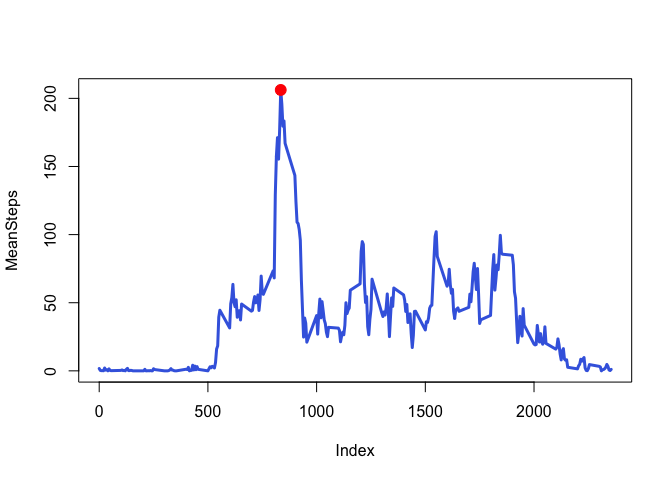
\includegraphics{RegressionModelProject_files/figure-latex/unnamed-chunk-6-1.pdf}

\begin{Shaded}
\begin{Highlighting}[]
\KeywordTok{par}\NormalTok{(}\DataTypeTok{mfrow=}\KeywordTok{c}\NormalTok{(}\DecValTok{2}\NormalTok{,}\DecValTok{2}\NormalTok{))}
\KeywordTok{plot}\NormalTok{(fitAMIntWt)}
\end{Highlighting}
\end{Shaded}

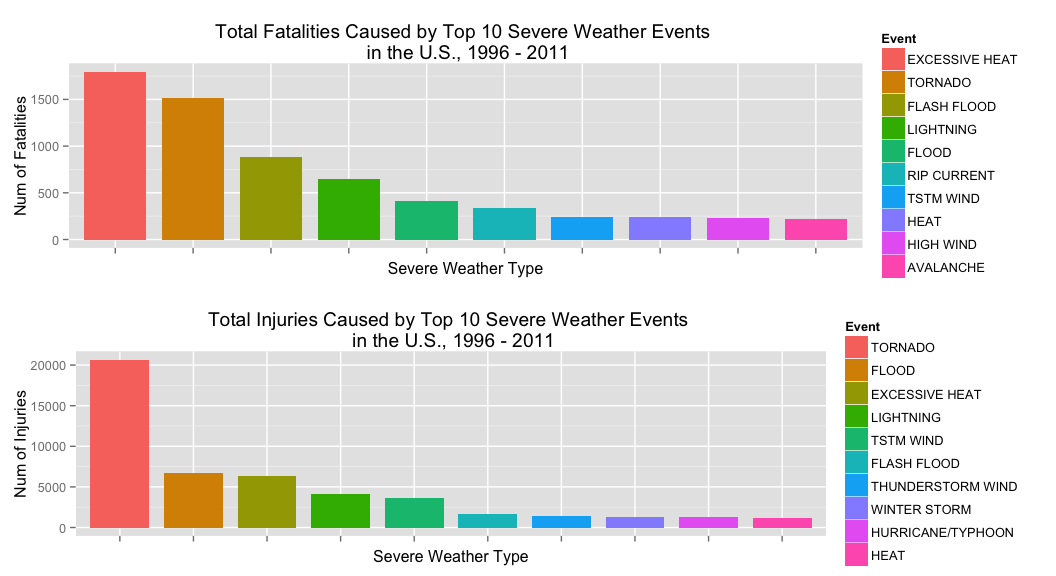
\includegraphics{RegressionModelProject_files/figure-latex/unnamed-chunk-7-1.pdf}

\end{document}
